\documentclass{beamer}

% Preamble {{{
\usepackage[ngerman]{babel}
\usepackage{epstopdf}
\usepackage[numbers,sort]{natbib}
\usepackage[T1]{fontenc}
\usepackage[utf8]{inputenc}
\usepackage{ifthen}
\usepackage{graphicx}
\usepackage{listings}
\usepackage{units}
\usepackage{tabularx}
\usepackage{arydshln}
\usepackage{caption} 
\captionsetup{format=hang}

\lstset{
	language=C,
	numbers=left,
	frame=single,
	basicstyle=\scriptsize,
	showstringspaces=false,
	captionpos=b,
	breaklines=true,
	breakatwhitespace=false,
	keywordstyle=\color{tgreen},
	commentstyle=\color{tblue},
	stringstyle=\color{tred}
}

\definecolor{tblue}{HTML}{729FCF}
\definecolor{tgreen}{HTML}{8AE234}
\definecolor{tred}{HTML}{EF2929}

\title{Selbst-adaptive Lastverteilung für DNS-Cluster}
%\subtitle{Verteidigung der Masterarbeit}
\author{Sebastian Menski\\\scriptsize{menski@uni-potsdam.de}}
\institute{Institut für Informatik\\Universität Potsdam}
\date{20. September 2012}

\setbeamertemplate{title page}{
    \vskip0pt plus 1filll
    \begin{centering}
        {\large\usebeamerfont{title}\usebeamercolor[fg]{title}\inserttitle}
        \vskip 5pt \par
        \hrule height 1pt \par
        \vskip 5pt \par
        {\normalsize\lineskip 0.75em
        \begin{tabular}[t]{c}
            \insertauthor
        \end{tabular}\par}
        \vskip 20pt \par
        {\small 
\includegraphics[width=2cm]{images/uni-logo}\\[20pt]\insertinstitute \par}
        \vskip 5pt \par
        {\footnotesize \insertdate \par}
    \end{centering}

    \vskip0pt plus 1filll
}

\setbeamertemplate{navigation symbols}{}

\setbeamertemplate{footline}{
 \begin{beamercolorbox}[ht=4ex,leftskip=.4cm,rightskip=.4cm]{author in head/foot}
  Sebastian Menski \hfill \inserttitle \hfill \insertframenumber/\inserttotalframenumber
 \end{beamercolorbox}
 \vspace*{0.1cm}
}

% }}}

\begin{document}

  % Intro {{{

  \frame{\thispagestyle{empty}\titlepage}
  \frame{\thispagestyle{empty}\frametitle{Gliederung}\tableofcontents{}}

  \newcommand{\mytitle}{}

  \newcommand{\mysection}[1]{
    \renewcommand{\mytitle}{#1}
    \section{#1}
    \frame{\thispagestyle{empty}
      \begin{center}
        \textcolor{beamer@blendedblue}{\LARGE\mytitle}
      \end{center}
    }
  }

  \newcommand{\myframe}[2][\empty]{
    \frame{\frametitle{\mytitle}
      \ifthenelse{\equal{#1}{\empty}}
      {#2}
      {\framesubtitle{#1}#2}
    }
  }

  \newcommand{\mybreakframe}[2][\empty]{
    \frame[allowframebreaks]{\frametitle{\mytitle}
      \ifthenelse{\equal{#1}{\empty}}
      {#2}
      {\framesubtitle{#1}#2}
    }
  }

  % }}}


  \mysection{Motivation} % {{{

    \myframe[Domain Name System (DNS)]{
        \begin{figure}
            \centering
            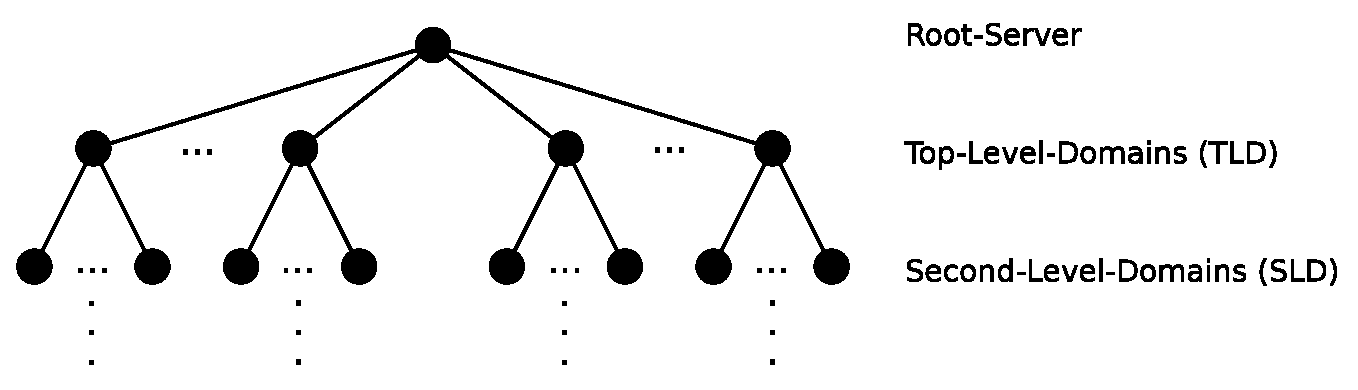
\includegraphics[width=\textwidth]{images/tree}
        \end{figure}
        \begin{itemize}
            \item Abbildung von Domain-Namen zu IP-Adressen
            \item Verteilte Datenbank
            \item Nameserver-Software: \textit{BIND}, \textit{NSD} und \textit{Microsoft DNS}
        \end{itemize}
    }

    \myframe[Domain Name System (DNS)]{
        \begin{figure}
            \centering
            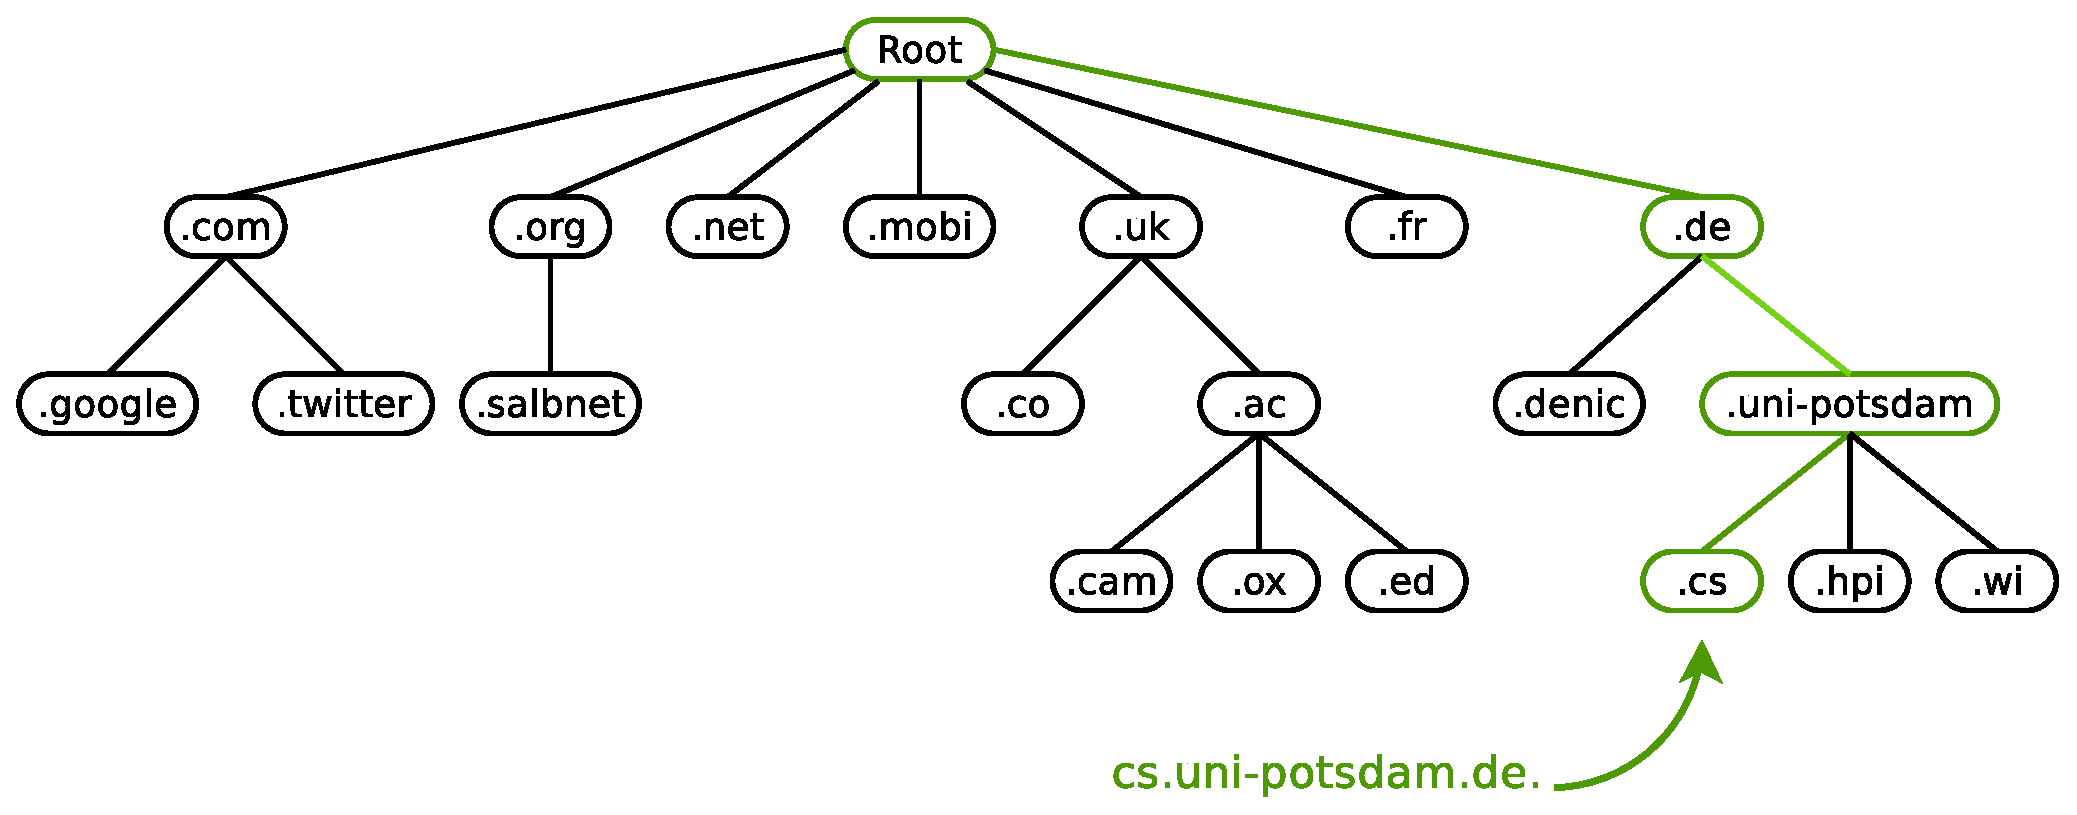
\includegraphics[width=\textwidth]{images/dns-tree-domains}
            \caption{Ausschnitt aus der DNS-Topologie}
            \label{fig:dns-topologie}
        \end{figure}
        
    }

    \myframe[DNS-Lastverteilung]{
        \begin{itemize}
            \item DNS-Round-Robin
            \item Server-Lastverteilung
            \item Anycast
            \item GeoIP
        \end{itemize}
    }

    \myframe[DNS-Round-Robin]{
        \begin{table}
            \begin{tabular}{|lccl|}\hline
                Domain & Klasse & Typ & Ziel \\\hline\hline
                uni-potsdam.de. & IN & NS & deneb.dfn.de. \\
                & IN & NS & ns.uni-potsdam.de. \\
                & IN & NS & schinkel.rz.uni-potsdam.de. \\
                & IN & NS & ws-kar1.win-ip.dfn.de. \\\hline
            \end{tabular}
        \end{table}
        \begin{itemize}
            \item Mehrere \texttt{NS}-Einträge für eine Domain
            \item Keine Ordnung
            \item Nameserver entscheidet über Ordnung in Antworten
            \item Oft wird Round-Robin gewählt
            \item Keine Beachtung der Last
            \item Keine Berücksichtigung von Ausfällen
        \end{itemize}
    }

    \myframe[DNS-Round-Robin]{
        \begin{table}
            \scriptsize
            \begin{tabular}{|lcccccl|}\hline
                Domain & Klasse & Typ & Priorität & Gewicht & Port & Ziel \\\hline\hline
                \_domain.\_udp.bsp.de & IN & SRV & 0 & 2 & 53 & ns1.bsp.de. \\
                & IN & SRV & 0 & 1 & 53 & ns2.bsp.de. \\
                & IN & SRV & 1 & 0 & 53 & ns3.bsp.de. \\\hline
            \end{tabular}
        \end{table}
        \begin{itemize}
            \item \texttt{SRV}-Einträge
            \item Ordnung und Gewichtung
            \item Definiert über Service und Protokoll
            \item Client wählt Nameserver aus
            \item Keine Beachtung der Last
        \end{itemize}
    }

    \myframe[Server-Lastverteilung]{
         \begin{figure}
             \centering
             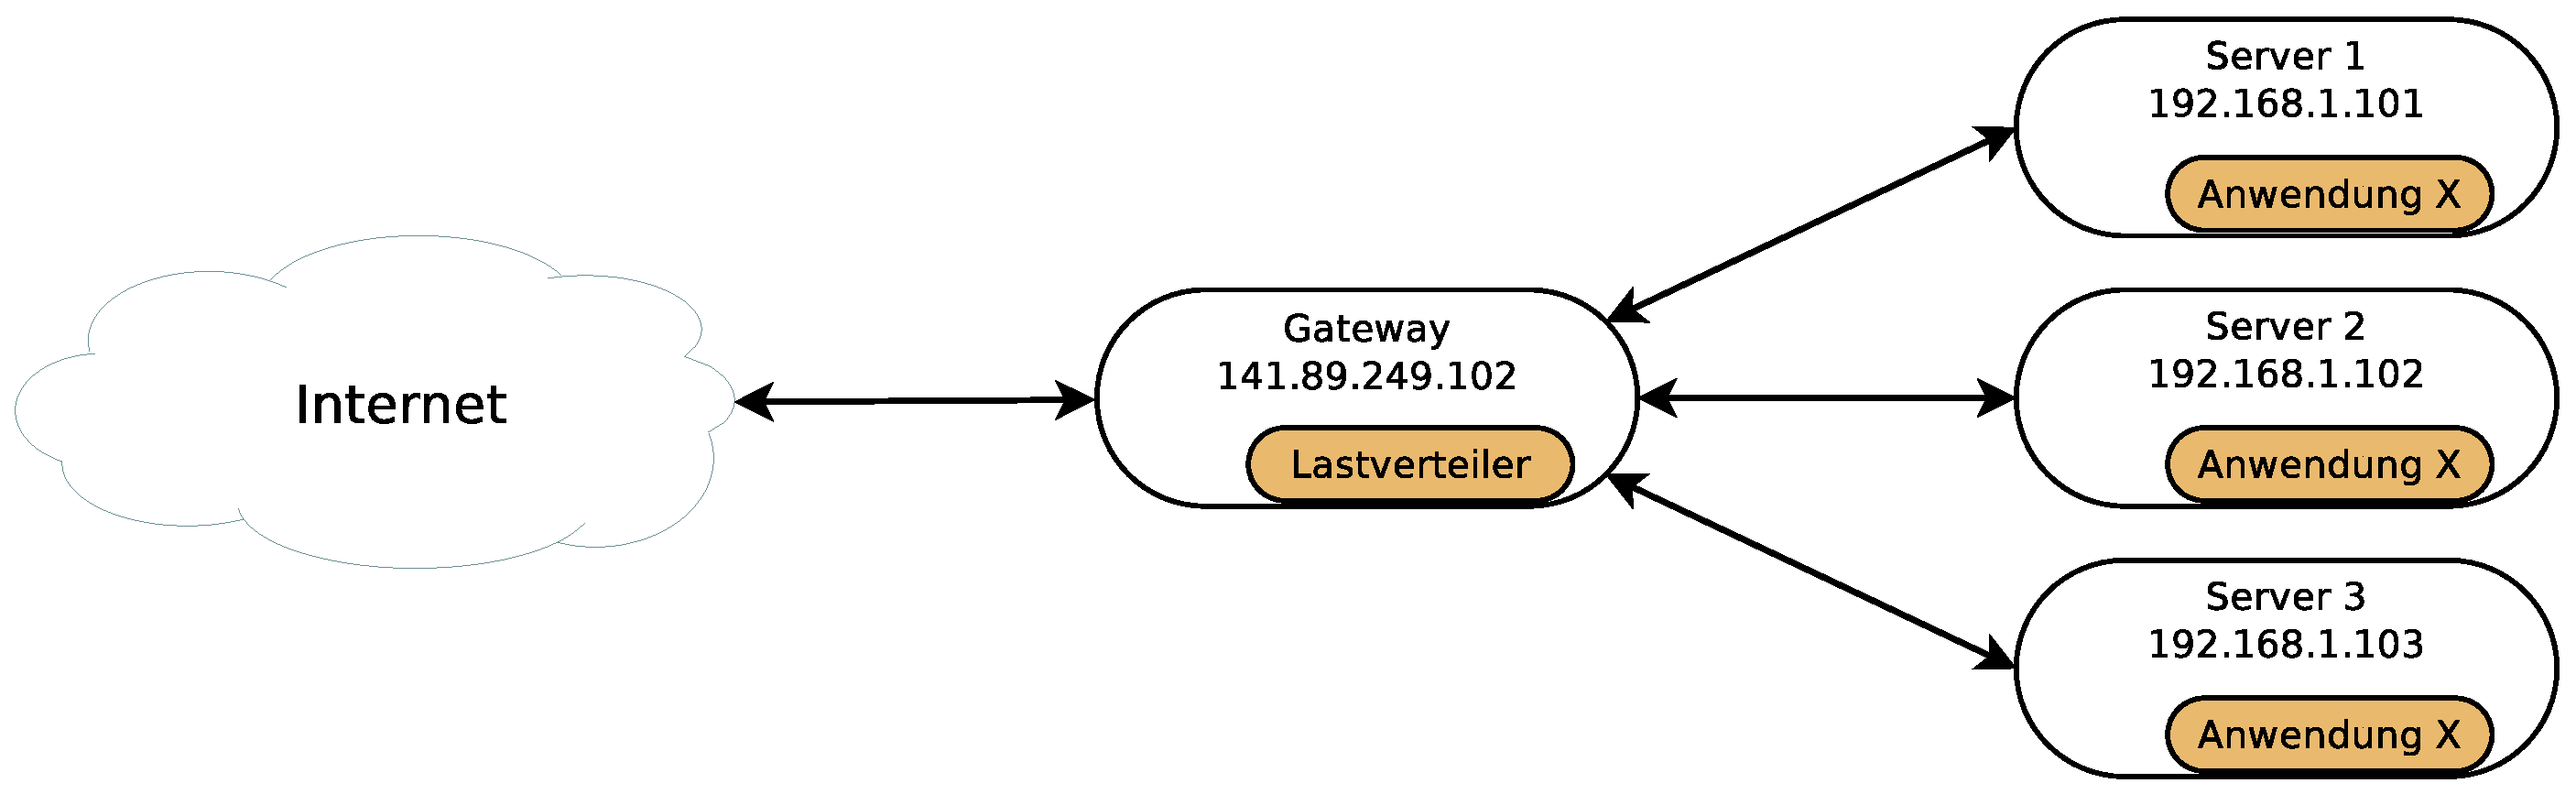
\includegraphics[width=9cm]{images/server-lastverteilung}
         \end{figure}
         \begin{itemize}
             \item Zentraler Ansatz
             \item Lastverteiler sendet Anfragen an Backend
             \item Verschiedene Algorithmen (Round-Robin, Least-Connection)
             \item Gewichtete Algorithmen
             \item Selten Beachtung von Last oder Ausfällen
             \item Beispiele: \textit{LVS} (Linux) und \textit{pf} (BSD)
         \end{itemize}

    }

    \myframe[Anycast \& GeoIP]{
        \textbf{Anycast}
        \begin{itemize}
            \item Mehrere Nameserver mit der gleichen IP-Adresse
            \item Server mit kürzester Route antwortet
        \end{itemize}
        \vspace{20pt}\par
        \textbf{GeoIP}
        \begin{itemize}
            \item Antwort abhängig von geografischer Lage
            \item Global Server Load Balancing
            \item Angepasste DNS-Antworten
        \end{itemize}
    }

    \myframe[Verwendung]{
        \begin{description}
            \item[Root-Server:] Anycast, Server-Lastverteilung
            \item[TLD:] Server-Lastverteilung, GeoIP, Anycast
            \item[SLD:] Server-Lastverteilung, DNS-Round-Robin
            \item[Lokal:] DNS-Round-Robin
        \end{description}
    }

    \myframe[DNS-Benchmarks]{
        \begin{itemize}
            \item \textit{queryperf}
                \begin{itemize}
                    \item \textit{BIND} \textit{contrib/}
                    \item Simples Log-Format (\texttt{www.bsp.de A})
                    \item Optionen:
                        \begin{itemize}
                            \item Zeitlimit oder Iterationen
                            \item Timeout und maximale Anzahl an ausstehenden Antworten
                        \end{itemize}
                \end{itemize}
            \item \textit{dnsperf}
                \begin{itemize}
                    \item Nominum Inc.
                    \item Simples Log-Format (\texttt{www.bsp.de. A})
                    \item Optionen:
                        \begin{itemize}
                            \item Zeitlimit oder Iterationen
                            \item Timeout und maximale Anzahl an ausstehenden Antworten
                            \item Anfragen pro Sekunde
                            \item Anzahl an Clients (Threads)
                        \end{itemize}
                \end{itemize}
            \item \textit{namebench}
                \begin{itemize}
                    \item Google
                    \item Vergleich von DNS-Servern
                    \item Keine eigenen Log-Dateien
                \end{itemize}
        \end{itemize}
    }

    \myframe[Fazit]{
        \begin{itemize}
            \item Server-Lastverteilung oft verwendeter Ansatz
            \item Häufig keine Beachtung der realen Last des Nameservers
            \item Benchmarks erzeugen keine realistischen Lastsituationen
        \end{itemize}

    }
  
    \myframe[Aufgabenstellung]{
      \begin{itemize}
          \item Erweiterung der Lastverteilung \textit{salbnet} für DNS
          \item Erweiterung des Benchmarks \textit{servload} für DNS
          \item Unterstützung des Nameservers \textit{BIND}
          \item Testmessungen auf dem \textit{IB}-Cluster des Instituts
      \end{itemize}
    }

  % }}} Motivation

  \mysection{salbnet} % {{{

    \myframe{
        \begin{itemize}
            \item Selbst-adaptive Lastverteilung
            \item Neuer LVS-Algorithmus
            \item Credit-basiert
            \item Round-Robin über alle Server mit Credits
            \item Unterstützt Ethernet und InfiniBand
        \end{itemize}
    }

    \myframe[Aufbau]{
        \begin{figure}
            \centering
            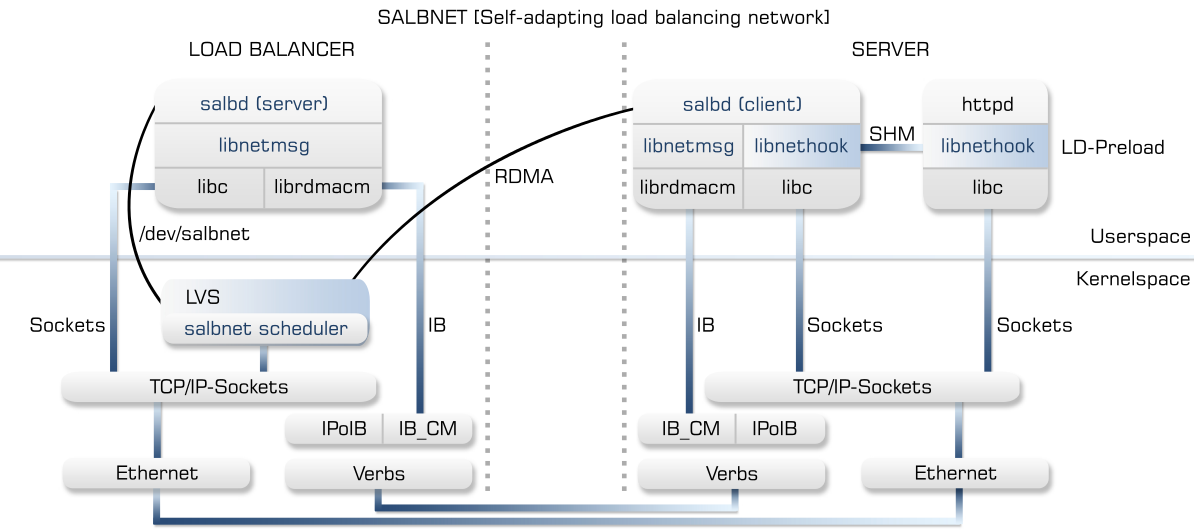
\includegraphics[width=\textwidth]{images/salbnet}
            \caption{\textit{salbnet}-Aufbau \cite{zinke2012}}
        \end{figure}
        
    }
    
    \myframe[Aufbau]{
        \begin{figure}
            \centering
            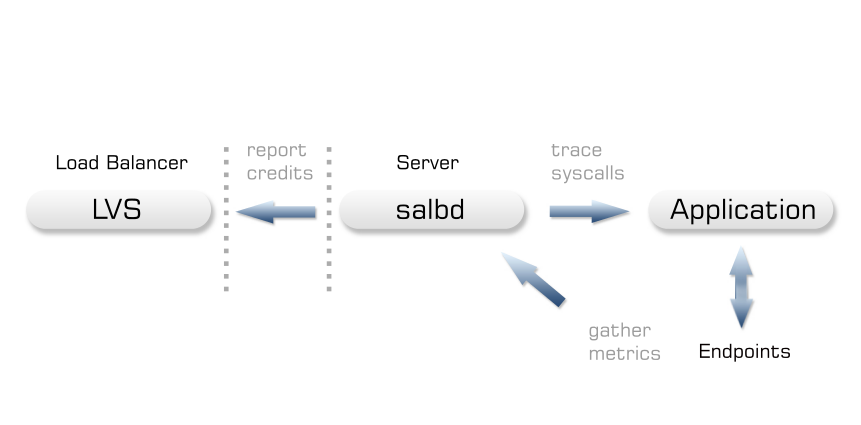
\includegraphics[width=\textwidth]{images/salbd-concept}
            \caption{\textit{salbd}-Konzept \cite{zinke2012}}
        \end{figure}
    }

    \myframe[Konzept - Metriken]{
        \begin{itemize}
            \item Last-Metrik
                \begin{itemize}
                    \item Ressourcenknappheit
                    \item Sammlung von Last-Daten
                    \item Abschätzung verbleibender Ressourcen
                \end{itemize}
            \item Verkehr-Metrik
                \begin{itemize}
                    \item Protokollierung des ein- und ausgehenden Netzwerkverkehrs
                    \item Differenz von ein- und ausgehenden Nachrichten
                    \item Anzahl zusätzlich möglicher Anfragen
                \end{itemize}
            \item Receive-Queue-Metrik
                \begin{itemize}
                    \item Menge an wartenden Anfragen
                    \item Füllstand der UDP-Receive-Queue
                    \item Restlicher Platz für weitere Anfragen
                \end{itemize}
        \end{itemize}
    }

    \myframe[Konzept - Kriterien]{
        \begin{itemize}
            \item Ein Credit = Eine weitere Anfrage
            \item Effiziente Berechnung
            \item Exakte Angabe möglicher Anfragen
            \item Applikationsunabhängigkeit
            \item Skalierbarkeit
        \end{itemize}
    }

    \myframe[Konzept - Auswahl]{
        \begin{itemize}
            \item Last-Metrik
                \begin{itemize}
                    \item[\textcolor{tgreen}+] Applikationsunabhängigkeit, Skalierbarkeit
                    \item[\textcolor{tred}{--}] Effiziente Berechnung, exakte Angabe möglicher Anfragen
                \end{itemize}
            \item Verkehr-Metrik
                \begin{itemize}
                    \item[\textcolor{tgreen}+] Applikationsunabhängigkeit, effiziente Berechnung
                    \item[\textcolor{tred}{--}] Skalierbarkeit, exakte Angabe möglicher Anfragen
                \end{itemize}
            \item Receive-Queue-Metrik
                \begin{itemize}
                    \item[\textcolor{tgreen}+] Applikationsunabhängigkeit, Skalierbarkeit, effiziente Berechnung, exakte Angabe möglicher Anfragen
                \end{itemize}
        \end{itemize}
    }

    \myframe[Konzept - Entwurf]{
        \textbf{Messwerte}
            \begin{tabular}{rl}
                $q_{max}$		  & maximale Kapazität der UDP-Receive-Queue\\
                $q_{current}$ &	aktuell belegter Speicherplatz in der UDP-Receive-Queue\\
                $p_{median}$  & Median der Paketgrößen in der UDP-Receive-Queue\\
            \end{tabular}
        \vspace{20pt}\par
        \textbf{Credits}
        \begin{equation*}
            p_{additional} = \frac{q_{max} - q_{current}}{p_{median}}
        \end{equation*}
    }


    \myframe[Konzept - Entwurf]{
        \textbf{Messwerte}
            \begin{tabular}{rl}
                $q_{max}$		  & maximale Kapazität der UDP-Receive-Queue\\
                $q_{current}$ &	aktuell belegter Speicherplatz in der UDP-Receive-Queue\\
                $p_{median}$  & Median der Paketgrößen in der UDP-Receive-Queue\\
                $p_{drop}$ & verworfene Anfragen seit der letzten Creditberechnung \\
            \end{tabular}
        \vspace{20pt}\par
        \textbf{Credits}
        \begin{equation*}
			Credits = \begin{cases}0 & p_{drop}>0\\ \frac{\displaystyle q_{max} - q_{current}}{\displaystyle p_{median}}
			  & \text{sonst}\end{cases}
		\end{equation*}
    }

    \begin{frame}[containsverbatim]
        \frametitle{\mytitle}
        \framesubtitle{Implementierung}
        $q_{max}$ - Maximale Kapazität der UDP-Receive-Queue
        \vspace{10pt}\par
        \begin{itemize}
            \item \texttt{/proc/sys/net/core/rmem\_default}
            \item Einmalige Bestimmung beim Start
            \item \texttt{fscanf}-Aufruf
        \end{itemize}
        \vspace{20pt}\par
		\lstinputlisting[lastline=2,numbers=none]{listings/proc-rmem.txt}
    \end{frame}

    \begin{frame}[containsverbatim]
        \frametitle{\mytitle}
        \framesubtitle{Implementierung}
        $q_{current}$ - Aktuell belegter Speicherplatz in der UDP-Receive-Queue
        \vspace{10pt}\par
        \begin{itemize}
            \item \texttt{/proc/net/udp}
            \item Bestimmung bei Credit-Berechnung
            \item \texttt{fscanf}-Aufruf
            \item Vergleich mit registrierter IP und Port
            \item Alternative: \texttt{Netlink}-Socket
        \end{itemize}
        \vspace{20pt}\par
		\lstinputlisting[numbers=none]{listings/proc-udp.txt}
    \end{frame}

    \begin{frame}[containsverbatim]
        \frametitle{\mytitle}
        \framesubtitle{Implementierung}
        $p_{drop}$ - Verworfene Anfragen seit der letzten Credit-Meldung
        \vspace{10pt}\par
        \begin{itemize}
            \item \texttt{/proc/net/snmp}
            \item Bestimmung bei Credit-Berechnung
            \item \texttt{fscanf}-Aufruf
            \item Anzahl verworfener Anfragen des kompletten Systems
            \item Alternative: \texttt{/proc/net/udp}, \texttt{Netlink}-Socket
        \end{itemize}
        \vspace{20pt}\par
		\lstinputlisting[numbers=none]{listings/proc-snmp.txt}
    \end{frame}

    \begin{frame}[containsverbatim]
        \frametitle{\mytitle}
        \framesubtitle{Implementierung}
        $p_{median}$ - Median der Paketgrößen in der UDP-Receive-Queue
        \vspace{10pt}\par
        \begin{itemize}
            \item \textit{BIND}: \texttt{recvmsg}-Aufruf
            \item \textit{salbnet}: \textit{libnethook} LD-Preload
            \item Rückgabewert = Größe der DNS-Nachricht
            \item Linux-Kernel: \texttt{struct sk\_buff}
        \end{itemize}
        \vspace{20pt}\par
		\lstinputlisting[firstline=9,lastline=12,numbers=none]{listings/strace.txt}
    \end{frame}

    \myframe[Implementierung]{
        \textbf{Experiment}
        \begin{enumerate}
            \item Senden von DNS-Nachrichten mit steigender Größe
            \item Auslesen von \texttt{/proc/net/udp}
            \item Empfangen des Pakets mit \texttt{recvmsg}
            \item Auslesen von \texttt{/proc/net/udp}
        \end{enumerate}
    }
    
    \myframe[Implementierung]{
        \textbf{Ergebnisse}
		\begin{table}
			\centering
			\begin{tabular}{|c|c|}\hline
				Receive-Queue & recvmsg \\\hline\hline
				376 & 12-64 \\
				504 & 65-192 \\
				632 & 193-320 \\
				760 & 321-448 \\
				888 &	449-576\\\hline
			\end{tabular}
		\end{table}
        \vspace{10pt}\par
        \textbf{Abschätzung}
		\begin{equation*}
			\text{Receive-Queue} = \lfloor (\text{recvmsg} + 63) / 128 \rfloor \cdot 128 + 376
		\end{equation*}
    }

    % }}} salbnet

  \mysection{servload} % {{{
    
  \myframe{
    \begin{itemize}
        \item HTTP-Benchmark
        \item $\sim$ 2000 Zeilen C-Code
        \item Wiedereinspielen von realen Logs
        \item Beachtung von User-Sessions und Zeitstempeln
        \item Modifikation des Logs (\textit{fast}, \textit{multiply}, \textit{peak}, \textit{score})
    \end{itemize}
  }

  \myframe[Ablauf]{
      \begin{enumerate}
          \item Aufruf: \texttt{servload url file [method] [factor]}
          \item Einlesen des Logs
          \item Modifikation des Logs
          \item Wiedereinspielen des Logs
          \item Erstellung der Statistik
      \end{enumerate}
  }

  \myframe[Konzept]{
    \begin{itemize}
        \item Unterstützung des \texttt{dns://} URL-Schemas
        \item Unterstützung des \textit{BIND}-Logformats
        \item Erzeugung valider DNS-Anfragen
        \item Verarbeitung von DNS-Antworten
        \item Erstellung DNS-spezifischer Statistiken
    \end{itemize}
  }

  \myframe[Implementierung]{
    \begin{itemize}
        \item Grundgerüst von \textit{servload} bereits auf DNS vorbereitet
        \item 2 neue Datenstrukturen
            \begin{itemize}
                \item \texttt{struct svl\_request\_dns}
                \item \texttt{struct svl\_statistic\_dns}
            \end{itemize}
        \item 6 neue Funktionen
            \begin{itemize}
                \item \texttt{svl\_request\_dns\_parse}
                \item \texttt{svl\_request\_dns\_response}
                \item \texttt{svl\_request\_dns\_header}
                \item \texttt{svl\_request\_dns\_body}
                \item \texttt{svl\_statistic\_dns\_print}
                \item \texttt{svl\_queue\_promote}
            \end{itemize}
    \end{itemize}

  }

  % }}} servload

  \mysection{Messungen} % {{{

  \myframe{
      \begin{itemize}
          \item Vergleich von \textit{Weighted-Round-Robin (wrr)} und \textit{salbnet} mit der
              \textit{Dynamic Pressure Relieve} Meldestrategie
          \item Benchmark: \textit{servload}
          \item Nameserver: \textit{BIND}
          \item Log:
              \begin{itemize}
                  \item Anonymisiertes \textit{BIND}-Log vom Nameserver
                      \texttt{haiti.cs.uni-potsdam.de}
                  \item Zeitraum: 27. September 2011 10:41 bis 2. Oktober 2011 6:25
                  \item Statistik: 1026 Sessions (IP-Adressen), 1.003.149 DNS-Anfragen, $\varnothing$ 2,41 Anfragen pro Sekunde
                  \item Ausschnitt: 29. September 2011 von 5:55 bis 6:00
                  \item Modifikation: \texttt{multiply} 400, 800 und 1600
              \end{itemize}
      \end{itemize}
  }

  \myframe[Umgebung]{
      \begin{figure}
          \centering
          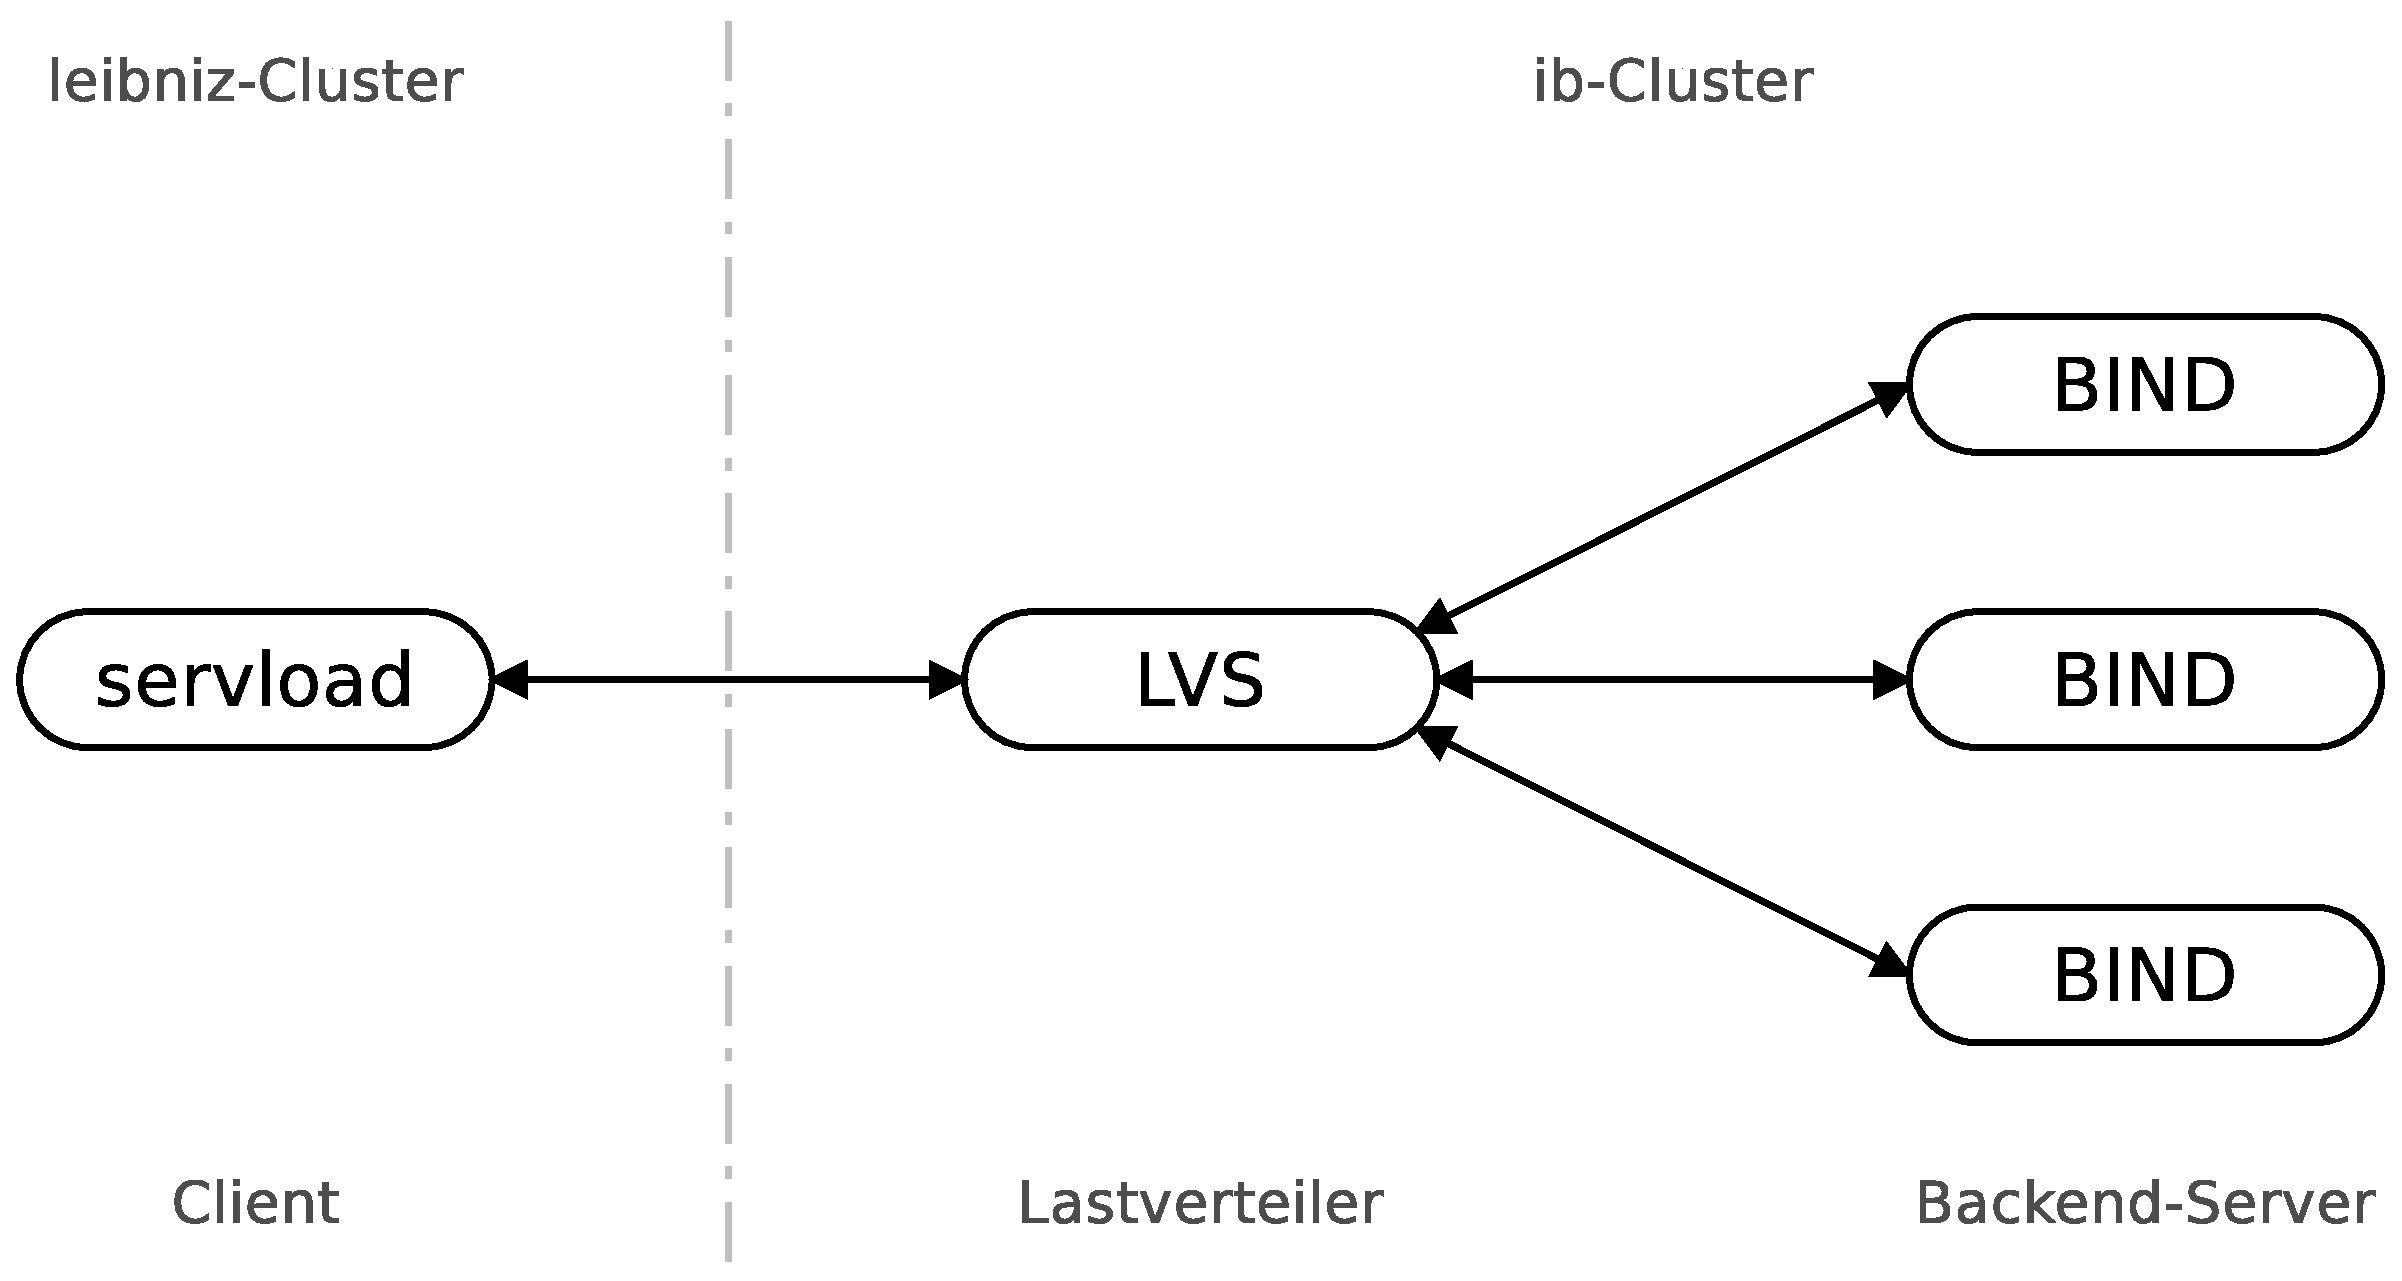
\includegraphics[width=\textwidth]{images/test-system}
      \end{figure}
  }

  \myframe[System]{
      \begin{description}
          \item[Client:] node015 -- Intel Xeon E5520 @ \unit[2,27]{GHz} (Quad-Core)\\\unit[12]{GB}
              RAM -- Debian 5.0.9
          \item[Lastverteiler:] ib1 -- 2 $\times$ AMD Opteron 244 @ \unit[1,8]{GHz}
              (Single-Core)\\\unit[4]{GB} RAM -- CentOS 5.7
          \item[Backend:] 
              \begin{itemize}
                  \item ib4 -- 2 $\times$ Opteron 244 @ \unit[1,8]{GHz} (Single-Core)\\\unit[4]{GB} RAM -- CentOS 5.7
                  \item ib6 -- Intel Pentium @ \unit[2,8]{GHz} (Single-Core)\\\unit[4]{GB} RAM -- CentOS 5.7
                  \item ib8 -- Intel Xeon 3040 @ \unit[1,86]{GHz} (Dual-Core)\\\unit[4]{GB} RAM -- CentOS 5.7
                  \item Receive-Queue: \unit[25165824]{Byte} (\unit[24]{MByte})
              \end{itemize}
      \end{description}
  }

  \myframe[Daten]{
      \begin{figure}
          \centering
          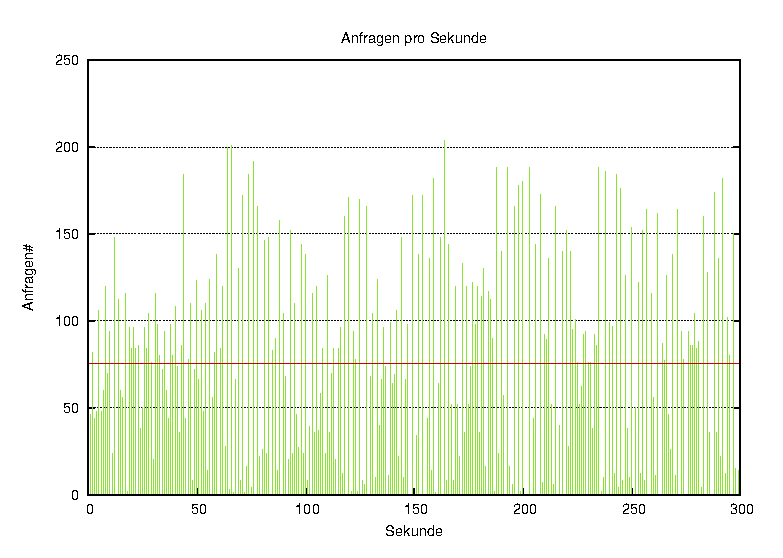
\includegraphics[width=9cm]{images/requests}
          \caption{Anfragen pro Sekunde für das Log vom 29. September 2011 von 5:55 bis 6:00}
      \end{figure}
  }

  \myframe[Ablauf]{
      \begin{itemize}
          \item Gewichte für wrr (Unixbench):\\ib4 -- 788, ib6 -- 623 und ib8 -- 1180 
          \item Ablauf: 51 Messungen je Algorithmus und Modifikation
          \item Insgesamt 306 Messungen
          \item Messwerte:
              \begin{itemize}
                  \item \textit{snmp}-Abfragen der ib1, ib4, ib6 und ib8
                  \item \textit{servload}-Statistiken
              \end{itemize}
      \end{itemize}
      \begin{table}
          \centering
          \small
          \begin{tabular}{|lrrrr|}\hline
              Faktor & Anfragen & Sessions & $\varnothing$ \nicefrac{Anfragen}{Sekunde} & max. \nicefrac{Anfragen}{Sekunde} \\\hline\hline
              1 & 22.594 & 33 & 75,31 & 204 \\
              400 & 9.037.600 & 13.200 & 30.125,33 & 81.600 \\
              800 & 18.075.200 & 26.400 & 60.250,67 & 163.200 \\
              1600 & 36.150.400 & 52.800 & 120.501,33 & 326.400 \\\hline
          \end{tabular}
          \caption{Kennzahlen des modifizierten Log-Intervalls}
      \end{table}
  }

  \myframe[Metriken]{
      \begin{itemize}
          \item CPU-Auslastung der Backend-Server in Prozent
          \item Anzahl der nicht beantworteten Anfragen (Timeout: eine Sekunde)
          \item Antwortzeit in Millisekunden
          \item Verbindungszeit in Millisekunden
      \end{itemize}
  }

  \myframe[Ergebnisse]{
      \begin{figure}
          \centering
          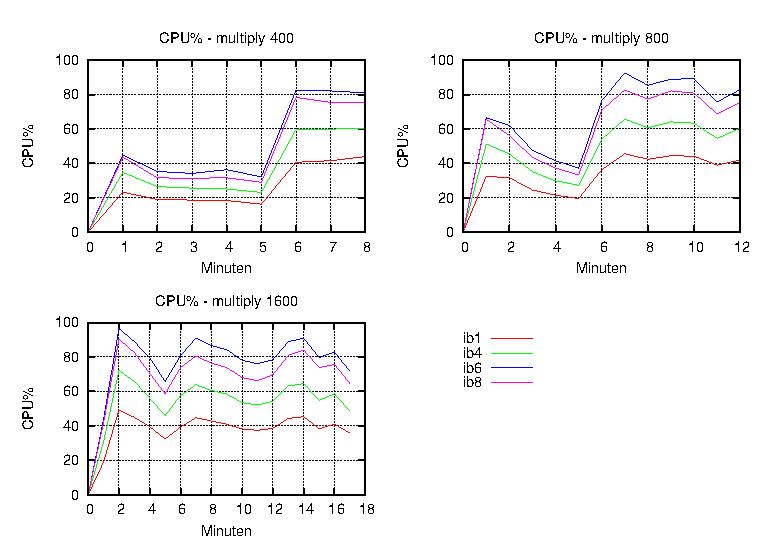
\includegraphics[width=9cm]{images/cpu-wrr}
          \caption{CPU Auslastung der Nodes ib1, ib4, ib6 und ib8 mit \textit{wrr} als
          Lastverteilungsalgorithmus}
      \end{figure}
  }
  
  \myframe[Ergebnisse]{
      \begin{figure}
          \centering
          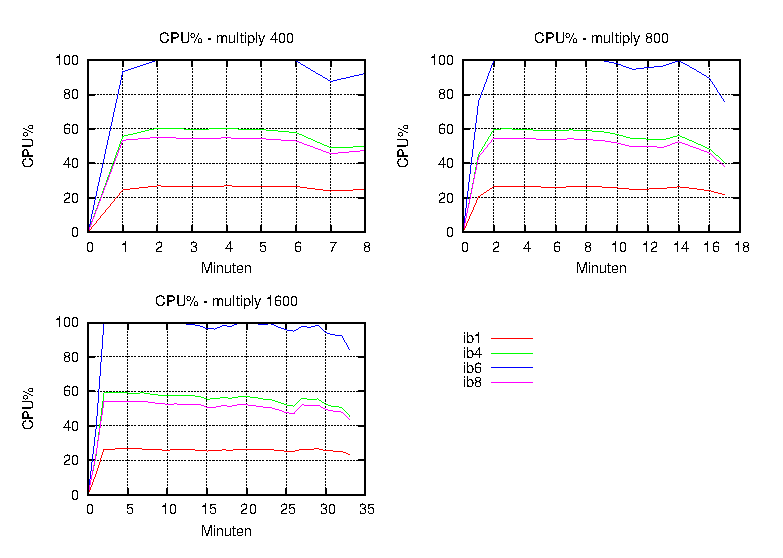
\includegraphics[width=9cm]{images/cpu-salbnet}
          \caption{CPU Auslastung der Nodes ib1, ib4, ib6 und ib8 mit \textit{salbnet} als
          Lastverteilungsalgorithmus}
      \end{figure}
  }

  \myframe[Ergebnisse]{
      \begin{figure}
          \centering
          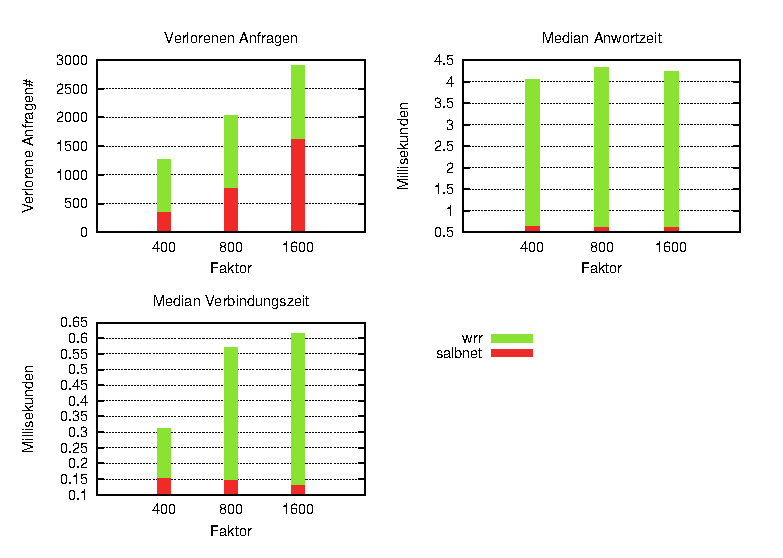
\includegraphics[width=9cm]{images/servload}
          \caption{Vergleich von \textit{wrr} und \textit{salbnet} für die Metriken: Verlorene Anfragen, Antwortzeit und Verbindungszeit}
      \end{figure}
  }

  \myframe[Ergebnisse]{
      \begin{table}
          \centering
          \begin{tabular}{|r|c|c|}\hline
              Faktor & \textit{wrr} & \textit{salbnet} \\\hline\hline
              400 & 1273,39 (182.727,4/427,5) & 343,16 (10.444,9/102,2)\\
              800 & 2038,53 (395.551,1/628,9) & 759,86 (30.414,0/174,4)\\
              1600 & 2910,16 (386.854,5/622,0) & 1612,78 (55.845,1/236,3)\\\hline
          \end{tabular}
          \caption{Anzahl der verlorenen Anfragen (Varianz/Standardabweichung)}
      \end{table}

      \begin{table}
          \centering
          \begin{tabular}{|r|c|c|}\hline
              Faktor & \textit{wrr} & \textit{salbnet} \\\hline\hline
              400 & 4,05 (0,95/0,98) & 0,64 (0,00/0,01)\\
              800 & 4,33 (2,50/1,58) & 0,61 (0,00/0,01)\\
              1600 & 4,24 (2,17/1,47) & 0,60 (0,00/0,02)\\\hline
          \end{tabular}
          \caption{Median Antwortzeit in Millisekunden (Varianz/Standardabweichung)}
      \end{table}
  }

  \myframe[Ergebnisse]{
      \begin{table}
          \centering
          \begin{tabular}{|r|c|c|}\hline
              Faktor & \textit{wrr} & \textit{salbnet} \\\hline\hline
              400 & 0,31 (0,00/0,05) & 0,15 (0,00/0,00)\\
              800 & 0,57 (0,05/0,22) & 0,14 (0,00/0,01)\\
              1600 & 0,61 (0,10/0,31) & 0,13 (0,00/0,00)\\\hline
          \end{tabular}
          \caption{Median Verbindungszeit in Millisekunden (Varianz/Standardabweichung)}
      \end{table}
  }


  % }}} Messungen

  \mysection{Fazit} % {{{
    
    \myframe[Zusammenfassung] {
        \begin{itemize}
            \item Unterstützung von DNS-Nachrichten über UDP für \textit{salbnet} und
                \textit{servload}
            \item \textit{salbnet} unterstützt den Nameserver \textit{BIND}
            \item \textit{salbnet} Abschätzung der Größe von DNS-Paketen ist wahrscheinlich auf Kernel 2.6.18
                beschränkt
            \item \textit{servload} unterstützt \textit{BIND}-Logs
            \item \textit{salbnet} ist in allen Messungen \textit{wrr} überlegen
            \item \textit{servload} kann große Mengen an Anfragen abarbeiten und senden
        \end{itemize}
    }

    \myframe[Ausblick]{
        \begin{itemize}
            \item salbnet
                \begin{itemize}
                    \item Kernel-Version unabhängige Abschätzung der Größe von DNS-Paketen
                    \item Verbesserung der Creditabschätzung
                    \item Unterstützung von DNS-Nachrichten über TCP
                    \item Portierung des \textit{salbnet}-Kernelmoduls
                    \item Verwendung von \textit{Netlink}-Sockets
                \end{itemize}         
            \item servload
                \begin{itemize}
                    \item Unterstützung von DNS-Nachrichten über TCP
                    \item DNS-Pipelining
                    \item DNS-Erweiterung (z.B. DNSSEC)
                \end{itemize}
        \end{itemize}
    }


  % }}} Fazit

  \section*{Im Internet} % {{{
    % TODO: Besserer Titel
    \myframe{
        \frametitle{Im Internet}
        \begin{columns}
            \column{9cm}
            \begin{itemize}
                \item \url{http://salbnet.org}
                \item \url{http://github.com/menski/master-thesis}
            \end{itemize}
        	\column{3cm}
		    
\includegraphics[width=3cm]{images/salbnet-logo}
        \end{columns}
    }

    % subsection Im Internet }}}

  % Appendix {{{

  \appendix{}
  \newcounter{finalframe}
  \setcounter{finalframe}{\value{framenumber}}
  \pagestyle{empty}
  \renewcommand{\mytitle}{Literaturverzeichnis}
  \frame[allowframebreaks]{\frametitle{\mytitle}
    \nocite{*}
    \bibliographystyle{dinat}
    \bibliography{references}
  }
  \setcounter{framenumber}{\value{finalframe}}

  % }}}

  \mysection{Anhang}
  \myframe[DNS-Nachrichtenformat]{
    \renewcommand{\arraystretch}{1.25}
    \begin{table}
        \centering
        \scriptsize
        \begin{tabularx}{\linewidth}{|X|X|X|X|X|X|X|X|X|X|X|X|X|X|X|X|} 
            0 & 1 & 2 & 3 & 4 & 5 & 6 & 7 & 8 & 9 & 10 & 11 & 12 & 13 & 14 & 15 \\\hline\hline
            \multicolumn{16}{|c|}{ID} \\\hline
            QR & \multicolumn{4}{c|}{Opcode} & AA & TC & RD & RA & \multicolumn{3}{c|}{Z} &
            \multicolumn{4}{c|}{RCODE} \\\hline
            \multicolumn{16}{|c|}{QDCOUNT} \\\hline
            \multicolumn{16}{|c|}{ANCOUNT} \\\hline
            \multicolumn{16}{|c|}{NSCOUNT} \\\hline
            \multicolumn{16}{|c|}{ARCOUNT} \\\hline
        \end{tabularx}
        \caption{Schematischer Aufbau des Headers einer DNS-Nachricht}
    \end{table}
    \renewcommand{\arraystretch}{1}
  }

  \myframe[DNS-Nachrichtenformat]{
      \renewcommand{\arraystretch}{1.25}
      \begin{table}
          \centering
          \scriptsize
          \begin{tabularx}{\linewidth}{|X|X|X|X|X|X|X|X|X|X|X|X|X|X|X|X|} 
              0 & 1 & 2 & 3 & 4 & 5 & 6 & 7 & 8 & 9 & 10 & 11 & 12 & 13 & 14 & 15 \\\hline\hline
              \multicolumn{16}{|c|}{} \\
              \multicolumn{16}{:c:}{QNAME} \\
              \multicolumn{16}{:c:}{} \\\hline
              \multicolumn{16}{|c|}{QTYPE} \\\hline
              \multicolumn{16}{|c|}{QCLASS} \\\hline
          \end{tabularx}
          \caption{Schematischer Aufbau des \textit{Question}-Abschnitts einer DNS-Nachricht}
      \end{table}
      \renewcommand{\arraystretch}{1}
  }

  \myframe[DNS-Nachrichtenformat]{
    \renewcommand{\arraystretch}{1.25} 
    \begin{table}
        \centering
        \scriptsize
        \begin{tabularx}{\linewidth}{|X|X|X|X|X|X|X|X|X|X|X|X|X|X|X|X|}
            0 & 1 & 2 & 3 & 4 & 5 & 6 & 7 & 8 & 9 & 10 & 11 & 12 & 13 & 14 & 15 \\\hline\hline
            \multicolumn{16}{|c|}{} \\
            \multicolumn{16}{:c:}{NAME} \\
            \multicolumn{16}{:c:}{} \\\hline
            \multicolumn{16}{|c|}{TYPE} \\\hline
            \multicolumn{16}{|c|}{CLASS} \\\hline
            \multicolumn{16}{|c|}{TTL} \\
            \multicolumn{16}{|c|}{} \\\hline
            \multicolumn{16}{|c|}{RDLENGTH} \\\hline
            \multicolumn{16}{:c:}{RDATA} \\
            \multicolumn{16}{:c:}{} \\\hline
        \end{tabularx}
        \caption{Schematischer Aufbau der \textit{Answer}/\textit{Authority}/\textit{Additional}-Abschnitte einer DNS-Nachricht}
    \end{table}
    \renewcommand{\arraystretch}{1}
  }

\end{document}
